\section{Entwicklung}
In diesem Kapitel wird die Entwicklung des digitalen Zwillings für die robocell beschrieben.
\dots

\dots

\dots

\dots

\dots
\dots
\subsection{Konzeptionierung des digitalen Zwilling}
Ziel dieses Kapitels ist es, eine grundlegende Basis für die Erstellung des digitalen Zwillings der robocell zu schaffen.
Dabei wird untersucht, welche Daten für die Modellierung erforderlich sind, wo diese herkommen und wie sie in (standardisierten) Teilmodellen der \acs{aas} strukturiert werden können.
\subsubsection{Identifikation relevanter Datenquellen}
Ein digitaler Zwilling basiert immmer auf einer Vielzahl unterschiedlicher Daten, die gemeinsam ein umfassendes digitales Abbild eines Assets ermöglichen. 
Dabei werden sowohl statische Informationen (z.B. Datenblätter oder Konstruktionsdaten) als auch dynamische Daten, die während des Betriebs einer Maschine anfallen, benötigt.

Im ersten Schritt gilt es daher, alle relevanten Datenquellen zu identifizieren.
In industriellen Umgebungen existieren hierfür typischerweise verschiedene Systeme zur Erfassung, Verwaltung und Speicherung von Maschinendaten.
Bei groninger übernimmt diese Funktion das \acs{plm}-System Agile, das eng mit dem \acs{erp}-System PSI Penta verknüpft ist.
Darin sind unter anderem Stücklisten, technische Spezifikationen, \acs{cad}-Dateien sowie allgemeine Dokumente hinterlegt, die die statische Grundlage  für den digitalen Zwilling bilden.

Neben den Informationen aus den Unternehmenssystemen spielen aber auch Laufzeitdaten, wie sie durch Sensoren oder Steuerungssysteme erzeugt werden, eine zentrale Rolle.
Da im Rahmen dieser Arbeit keine reale Maschine angebunden ist, werden diese Daten simuliert.
Hierfür wird eine in node.js entwickelte Anwendung eingesetzt, die sowohl Prozess- als auch Betriebsdaten generiert. 
Ergänzend dazu wird ein Maschinensimulator verwendet, der einen PackML-Zustandsautomaten abbildet und typische Maschinenzustände sowie deren Übergänge simuliert. 
Beide Komponenten stehen als Docker Container zur Verfügung und stellen die Daten über einen \acs{opcua} Server bereit, wodurch eine realitätsnahe Datenbasis geschaffen wird.
\subsubsection{Auswahl geeigneter Teilmodelle}
Aufbauend auf den zuvor betrachteten Informationsquellen gilt es nun zu entscheiden, welche Aspekte der Maschine im digitalen Zwilling abgebildet werden sollen.
Dabei werden die Informationen in unterschiedlichen Submodellen der \acs{aas} strukturiert.

Als Orientierung dienen die von der \acs{idta} bereitgestellten Submodel Templates \cite{idtaTemplates}, die bereits viele typische Anwendungsfälle standardisiert abdecken.
Diese sind jeweils in einer Spezifikation der \acs{idta} definiert.
Darüber hinaus besteht jedoch auch die Möglichkeit, eigene Submodelle zu entwerfen, die gezielt auf projektspezifische Anforderungen zugeschnitten sind.
Diese können entweder vollständig neu konzipiert oder aus bestehenden Vorlagen abgeleitet werden.

Die konkrete Auswahl der Submodelle in dieser Arbeit orientiert sich hauptsächlich an typischen Industrie 4.0-Anwendungsfällen, die unter anderem auf der Website der \acs{idta} dokumentiert sind \cite{idtaUseCases}.
Diese Anwendungsfälle zeigen auf, welche Submodelle in der Praxis besonders relevant sind.
Eines der wichtigsten ist vermutlich das digitale Typenschild.
Daneben wurden aber auch projektspezifische Anforderungen berücksichtigt, die sich aus den verfügbaren Daten sowie dem fachlichen Austausch mit Industriepartnern wie Wittenstein ergaben.


Ein wesentlicher Vorteil der \acs{aas} besteht darin, dass die Auswahl der Submodelle flexibel ist.
Sie können sukszessive ergänzt, angepasst oder auch wieder entfernt werden.
Es werden im Folgenden deshalb zunächst nur die wichtigsten, in diesem Projekt eingesetzten Submodelle betrachtet, die in späteren Anwendungsfällen gezielt erweitert werden.

Die nachfolgende Tabelle gibt einen Überblick über die initiale Auswahl dieser Submodelle, ihre typischen Inhalte sowie deren Standardisierung.

% Wie erfolgt die Auswahl? sss

%Nachfolgende Tabelle gibt einen Überblick über die wichtigsten, in diesem Projekt eingesetzten Submodelle sowie ihrer Inhalte.
%Die bereits veröffentlichten Modelle sind dabei jeweils in einer Spezifikation der \acs{idta} standardisiert.

%\newpage
{\small
\begin{longtblr}[
    label = tab:Submodelle,
    entry = Submodelle mit typischen Inhalten,
    caption = {Submodelle mit typischen Inhalten}
  ]{
    colspec = {l l X[c]},
    rowhead = 1,
    vlines,
    hline{1-11} = {-}{},
    }
    \textbf{Submodell}                                   & \textbf{Typische Inhalte}                            & \textbf{Standardisierung} \\
    Typenschild                                          & \makecell[l]{Hersteller \\ Seriennummer \\ Adressinformationen}                  & IDTA 02006-3-0 \cite{SpezifikationTypenschild} \\
    Dokumentation                                     & \makecell[l]{Allgemeine Dokumente \\ Betriebsanleitungen \\ Projektzeichnungen}             & IDTA 02004-1-2 \cite{SpezifikationDokumentation} \\
    3D-Modelle                                           & Konstruktionsmodelle                & IDTA 02026-1-0 \cite{Spezifikation3DModelle}\\*
    Technische Daten                                     & \makecell[l]{Generelle Informationen \\ Technische Eigenschaften }                       & IDTA 02003 \cite{SpezifikaitonTechnischeDaten}\\*
    \acs{bom}                                     &  \makecell[l]{Strukturierte Stücklisten \\ Komponentenbeziehungen }                    & IDTA 02011-1-1 \cite{SpezifikationHierachischeStrukturen}\\*
    Wartung                                              &  \makecell[l]{Wartungsinformationen \\ Wartungsintervalle \\ }          & -  \\*
    Prozessdaten                                         &  \makecell[l]{Messwerte}             & - \\*
    Zeitreihendaten                                       &  \makecell[l]{Zeitreihen }             & IDTA 02008-1-1 \cite{SpezifikationTimeSeriesData}    \\*
    Kontrollkomponente                                   &  \makecell[l]{Betriebsmodi \\ Schnitstelle zur Automatisierung }             & - \\      
\end{longtblr}
}





\subsection{Modellierung mit der AAS}
In diesem Kapitel wird erläutert, wie die zuvor ausgewählten Submodelle mit konkreten Daten befüllt werden können und welche Aspekte bei der Modellierung beachtet werden müssen.
Zudem wird gezeigt, wie die erstellte \acs{aas} mit Hilfe einer Test Engine auf eine korrekte und vollständige Struktur überprüft werden kann. 
\subsubsection{Umsetzung mit dem Package Explorer}
Für die manuelle Erstellung der \acs{aas} wird der Package Explorer eingesetzt.
Er erlaubt eine eine intuitive Modellierung aller relevanten Elemente und erleichtert so den strukturierten Aufbau der \acs{aas}.

Bevor die gewünschten Submodelle hinzugefügt werden können muss zuerst eine neues \acs{aas}-Paket erstellt werden.
Dazu kann im Package Exporer eine neue Umgebung geöffnet werden, die als Container für die Inhalte eines Assets dient.
Im Anschluss kann eine neue \acs{aas} hinzugefügt werden, die allgemeine Informationen sowie assetspezifische Daten enthält.

Neben der Auswahl des Asset-Typs (Instanz oder Typ) spielt insbesondere die eindeutige Identifikation eine wichtige Rolle.
Das Asset wird über eine globalAssetId identifiziert, während die \acs{aas} selbst eine eigene ID sowie eine idShort erhält.
Es bietet sich an, hierfür zunächst Beispiel-IDs zu verwenden. Diese können direkt im Package Explorer generiert werden.
Dies ist besonders wichtig für den späteren Austausch der \acs{aas} sowie das systemweite Auffinden innerhalb eines Industrie 4.0-Ökosystem.
Darüber hinaus besteht ebenfalls die Möglichkeit, ein Thumbmail in Form einer Datei (z.B. png oder jpeg) zu hinterlegen.

Im nächsten Schritt können die benötigten Submodelle hinzugefügt werden. 
Auch diese können als Instanz oder Typ angelegt werden.
Dabei besteht die Möglichkeit, entweder ein leeres Submodell manuell mit verschiedenen Submodellelementen zu erstellen oder auf ein vorhandenes Submodel Template zurückzugreifen.
Letztere können als AASX-Datei, beispielsweise über das Repository der \acs{idta} \cite{idtaTemplates}, heruntergeladen und anschließend über ein sogenanntes Auxiliary AAS in die Umgebung geladen werden.
Sie stehen dann zur Verfügung und können in die \acs{aas} kopiert werden.

Nachdem alle Submodelle erstellt bzw. eingebunden sind, müssen diese mit den entsprechenden Inhalten gefüllt werden.
Hierzu können konkrete Werte, Dateien oder Referenzen direkt in den jeweiligen Submodellelementen eingetragen bzw. eingebettet werden.
Besonders bei der Verwendung von Templates muss darauf geachtet werden, dass die Struktur dieser nicht verändert wird, da dies sonst zu Abweichungen von der Spezifikation führen kann.
Eine Übersicht über die Modellierungsumgebung im Package Explorer mit einem geöffneten Submodell ist in Abbildung \ref{fig:BearbeitungsansichtPackageExplorer} dargestellt.

\begin{figure}[htbp]
    \centering
    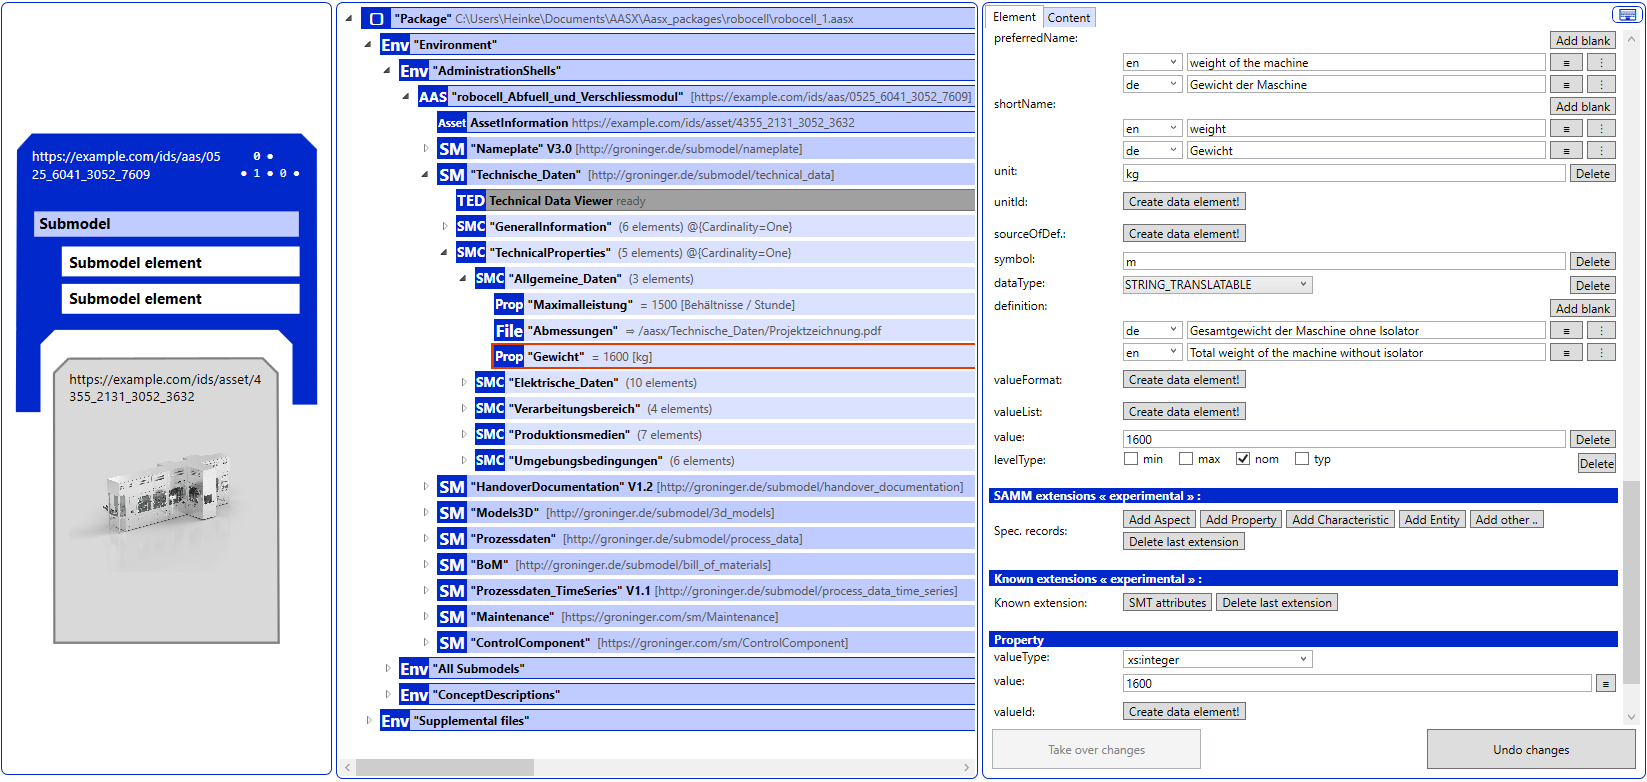
\includegraphics[width=1\textwidth]{Bilder/ModellierungAAS/neu.PNG}
    \caption{Bearbeitungsansicht eines Submodells im Package Explorer}
    \label{fig:BearbeitungsansichtPackageExplorer}
\end{figure}

Zur Gewährleistung einer einheitlichen semantischen Beschreibung können einzelne Elemente innerhalb eines Submodells mit einer semanticId versehen werden.
Diese verweist entweder auf externe Standards oder auf lokale Concept Descriptions innerhalb der AAS-Umgebung.
Eine Concept Description kann manuell erstellt oder über den ECLASS-Standard eingebunden werden.
Der Package Explorer bietet hierfür eine erweiterte Funktion, bei der sich vorgefertigte ECLASS-Kataloge importieren lassen.
Die enthalten Begriffe können direkt im Package Explorer dursucht, ausgewählt und dem enstprechenden Submodellelementen zugewiesen werden.

Sobald alle gewünschten Submodelle mit Inhalten gefüllt und semantisch beschrieben sind, kann die \acs{aas} gespeichert und exportiert werden.
In diesem Projekt erfolgt dies bevorzugt im AASX-Format, das sich als standardisierte Austauschform für die \acs{aas} etabliert hat und eine einfache Weitergabe oder Validierung ermöglicht.




\subsubsection{Validierung}
Nach der Erstellung sollte eine Überprüfung der Konformität der \acs{aas} erfolgen.
Hierzu wird eine von der \acs{idta} bereitgestellte Test Engine eingesetzt \cite{TestEngine}. 
Diese kann direkt mit pip, dem Paktemanager von Python, installiert und anschließend über die Kommandozeile genutzt werden.

Mit dem Befehl \texttt{aas\_test\_engines check\_file robocell.aasx} kann nun die zuvor erstellte AASX-Datei der robocell validiert werden.
%Mit dem Befehl: aas_test_engines check_file my_aas.aasx kann eine AASX-Datei validiert werden.
% \begin{verbatim}
% aas_test_engines check_file robocell.aasx
% \end{verbatim}
Dabei wird zunächst geprüft, ob die AASX-Datei formal korrekt aufgebaut ist, insbesondere hinsichtlich der internen Struktur und ihrer Beziehungen.
Anschließend erfolgt die Kontrolle der enthaltenen \acs{aas} gegen die Metamodell-Spezifikationen der \acs{idta} (Teil 1 \cite{SpezifikationPart1} und 3a \cite{SpezifikationPart3a}).
Zuletzt erfolgt ein Abgleich der Submodelle mit ihren entsprechenden Submodel Templates.
Wenn im ganzen Prozess keine Fehler oder Abweichungen gefunden werden, folgt eine entsprechende Bestätigung der Test Engine (siehe Abbildung \ref{fig:KonsolenausgabeTestEngine}).

\setlength{\fboxsep}{0pt}
\begin{figure}[htbp]
    \centering
    \fcolorbox{black!60}{white}{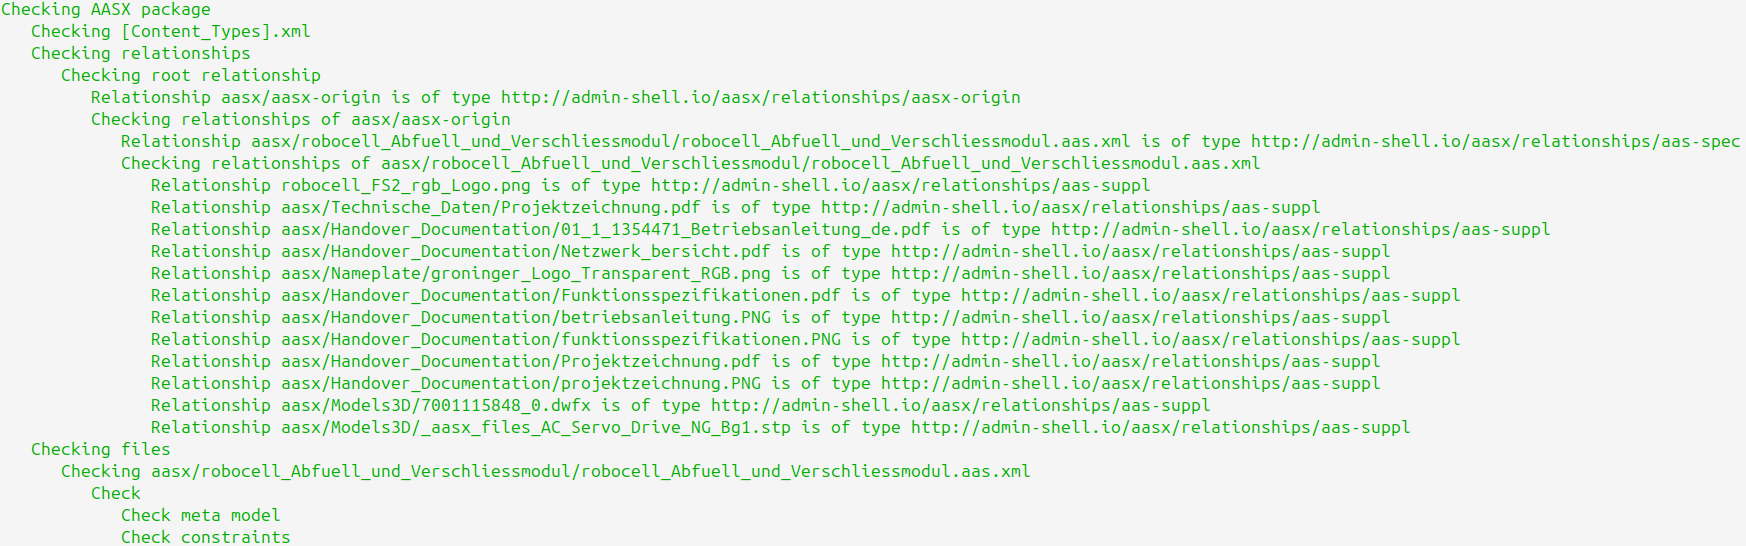
\includegraphics[width=0.99\textwidth]{Bilder/testEngineSuccess.PNG}}
    \caption{Konsolenausgabe nach erfolgreicher Validierung}
    \label{fig:KonsolenausgabeTestEngine}
\end{figure}

\subsection{Technische Integration}
\subsubsection{Bereitstellung der Verwaltungsschalen}
\subsubsection{Datenzugriff über standardisierte Schnittstellen}



\newpage
\subsubsection{Integration von Echtzeitdaten über OPC UA}
Nach der Erstellung einer statischen \acs{aas} für die robocell gilt es nun, diese um dynamische Informationen zu erweitern.
Diese sind essenziell, um den aktuellen Zustand einer Maschine abbilden zu können.
Die Datenbasis bilden die beiden zuvor vorgestellten Anwendungen, die Maschinen- bzw. Sensordaten über einen OPC UA Server bereitstellen.
% Auf die konkrete Simulation dieser Daten soll in dieser Arbeit allerdings nicht weiter eingegangen werden.

% Dennoch ist es sinnvoll, einmal die Struktur der bereitgestellten Daten zu betrachten.

% Zur Analyse kann ein OPC UA Client genutzt werden, z.B. UA Expert, mit dem alle verfügbaren Datenpunkte (Nodes) eingesehen werden können.
% Die Daten werden in einer hierarchischen Struktur bereitgestellt, wie sie in Abbildung \ref{fig:opcua_serverstruktur} zu erkennen ist.
% Jede Node besitzt dabei einen NamespaceIndex sowie eine eindeutige NodeId (siehe Abbildung \ref{fig:opcua_pressure_node}), über die das jeweilige Objekt identifiziert werden kann.

% \begin{figure}[htbp]
%     \centering
%     \begin{minipage}[t]{0.25\textwidth}
%         \centering
%         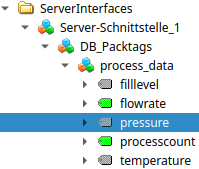
\includegraphics[width=\textwidth]{Bilder/OPCUA/serverstruktur.png}
%         \caption{OPC UA Serverstruktur}
%         \label{fig:opcua_serverstruktur}
%     \end{minipage}
%     \hspace{0.2\textwidth} % Abstand zwischen den Bildern
%     \begin{minipage}[t]{0.4\textwidth}
%         \centering
%         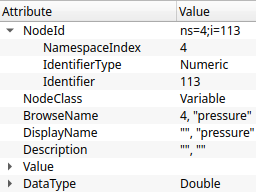
\includegraphics[width=\textwidth]{Bilder/OPCUA/pressure_node.png}
%         \caption{Detailansicht der Node \texttt{pressure}}
%         \label{fig:opcua_pressure_node}
%     \end{minipage}
% \end{figure}

Die technische Integration in die \acs{aas} wird im Folgenden am Beispiel des Submodells Prozessdaten erläutert.
Innerhalb dieses Submodells existieren verschiedene Properties, die jeweils bestimmte Werte, wie beispielsweise den Druck, repräsentieren (siehe Abbildung \ref{fig:UMLSubmodellProcessData}). 
Diese Properties sollen im weiteren Verlauf dynamisch mit den simulierten Werten, die über \acs{opcua} bereitgestellt werden, aktualisiert werden.

\begin{figure}[htbp]
    \centering
    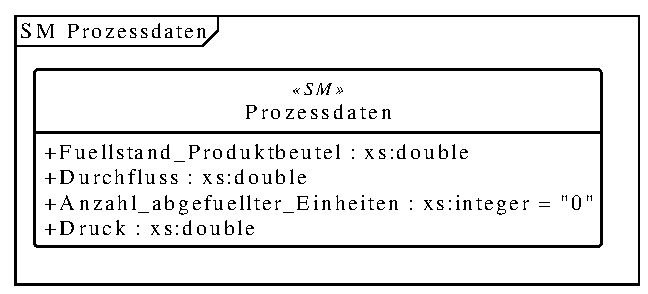
\includegraphics[width=0.5\textwidth]{Bilder/UML/submodel_processdata.pdf}
    \caption{Klassendiagramm des Submodells Prozessdaten}
    \label{fig:UMLSubmodellProcessData}
\end{figure}

Das Eclipse BaSyx Projekt stellt hierfür eine weitere Komponente bereit, die sogenannte Databridge \cite{BaSyxDatabridge}.
Diese steht, wie alle anderen Komponenten auch, als Docker Container zur Verfügung und ermöglicht die Anbindung verschiedenster Datenquellen an eine \acs{aas}.
Sie unterstützt eine Vielzahl von Protokollen, darunter insbesondere auch \acs{opcua} oder MQTT.
Dabei dient sie als Vermittler zwischen einem Datenendpunkt, in diesem Fall einem \acs{opcua} Server und einem Submodell innerhalb der \acs{aas}.

Die Konfiguration der Databridge erfolgt über mehrere JSON-Dateien.
In der Datei routes.json werden sowohl die Datenquelle als auch die Datensenke definiert.
Die Aktualisierung der Daten erfolgt dabei ereignisbasiert anhand eines Event-Triggers.
Dies entspricht einer klassischen Subscription, bei der die Databridge automatisch benachrichtigt wird, sobald sich der Wert des OPC UA Servers ändert.




\subsubsection{Verarbeitung von Zeitreihendaten}

\subsection{Anwendungsfall Digitaler Produktpass}
\subsubsection{Beschreibung}
\subsubsection{Umsetzung mit dem Teilmodell Carbon Footprint}
\subsection{Anwendungsfall automatisierte Generierung von AAS}
\subsubsection{Erstellen von Submodell-Templates}
\subsubsection{Befüllen der Templates mit strukturierten Daten}
\subsubsection{Bereitstellen der AAS über die Rest API}
\subsubsection{Potenziale des KI-Einsatzes}